\documentclass[10pt]{article}
\usepackage{icmlko}

\icmlmeta{IP 파운데이션 월드모델}{236}{공짜는 셋 다 함정이었다}{노트 235가 모바일의 빈칸을 가리켰다. 채우러 갔더니 API 호출 없이 522건을 채울 수 있었고, 세 번 거르니 0 이 됐다}

\begin{document}

\twocolumn[
\icmlheader

\begin{abstract}
노트 235가 ``모바일 유보 150건은 검색 축이 없는 행이고 그것을 채우면
노트 220의 천장 $+$0.0669 에 닿는다''를 남겼다. 채우러 갔다가 더 싼 것을
먼저 봤다 --- \textbf{미수집 레코드 중 522건은 API 호출이 0 이다.}
키워드가 이미 다른 레코드에 쓰여 받아 놓은 계열이 있기 때문이다
(\texttt{targets()} 가 ``같은 검색어를 두 번 사지 않는다''로 걸러 낸
것들이다). \textbf{세 번 걸렀더니 0 이 됐다.} ① \textbf{67\% 가 계열
질의다} --- 노트 222가 정의로 결측 처리한 바로 그것이라 306건을 뺀다.
남은 216건은 \texttt{(자막) 도굴왕} 대 \texttt{(더빙) 도굴왕} 처럼
\emph{같은 작품의 다른 판}이라 계열을 공유하는 것이 옳아 보였다.
② \textbf{채워 보니 판이 내려간다} --- F23 $+$0.4524 $\to$ $+$0.4490 ·
F18 $+$0.4409 $\to$ $+$0.4370 이다. 왜인지 쟀다: \textbf{같은 작품의 두
판이 라벨은 크게 다르다.} 애니 공유 쌍 96개에서 쌍 안 라벨 sd 가 도메인
sd 의 \textbf{32\%} 이고 \textbf{26\% 는 절반을 넘는다}(자막 0.85 대
더빙 2.40 · 0.00 대 1.51). \textbf{축을 같게 만들면 그 둘 사이를 못 가르고,
판정치가 순위이므로 그것이 곧 손해다.} ③ \textbf{그리고 정작 모바일은
216건에 하나도 없다} --- 모바일의 재사용 가능 14건이 전부 다른 작품이다.
\textbf{이 조사를 시작하게 한 도메인이 정확히 0 을 받는다.} 되돌렸다.
남는 것은 노트 235가 이미 가리킨 것뿐이다 --- \textbf{모바일 영문 제목
690건의 음역}이고, 그것은 공짜가 아니다.
\end{abstract}
]

\begin{figure*}[t]
\centering
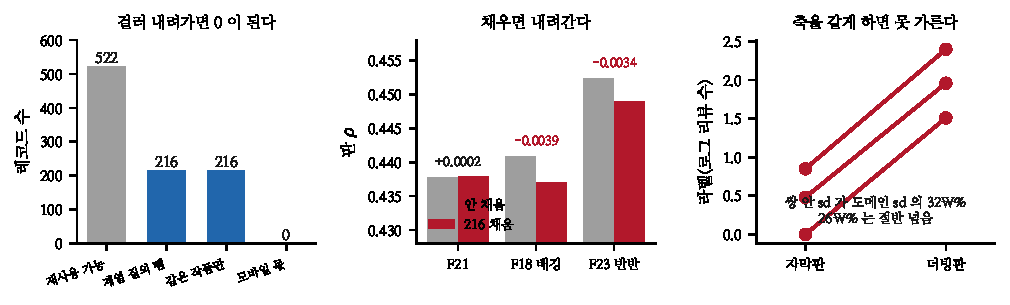
\includegraphics[width=\textwidth]{figs/freetrap.pdf}
\caption{왼쪽 --- 걸러 내려가면 0 이 된다. 가운데 --- 216 을 채워도
판이 내려간다. 오른쪽 --- 같은 작품인데 라벨이 크게 다르다.}
\end{figure*}

\section{첫째 거름 --- 계열 질의}

\begin{table}[t]
\centering\tsize
\caption{API 호출 0 으로 채울 수 있는 레코드.}
\begin{tabular}{lrrr}
\toprule
& 재사용 가능 & 계열 질의 & 남는 것 \\
\midrule
애니 & 363 & 315 (87\%) & 97 \\
도서 & 135 & 15 (11\%) & 118 \\
\textbf{모바일} & \textbf{14} & \textbf{14 (100\%)} & \textbf{0} \\
웹툰 · 게임 · 펀딩 & 10 & 7 & 3 \\
\midrule
합계 & \textbf{522} & 351 (67\%) & \textbf{216} \\
\bottomrule
\end{tabular}
\end{table}

\claimx{\textbf{67\% 가 계열 질의다} --- 노트 222가 ``계열 안 여러
레코드가 같은 값을 받으면 작품을 못 가른다''로 결측 처리한 바로
그것이다.}{\textbf{\texttt{targets()} 의 ``같은 검색어를 두 번 사지
않는다''가 API 절약이 아니라 타당성 규칙이었다} --- 그때는 그걸 모르고
썼다.}

\section{둘째 거름 --- 같은 작품인데도 안 된다}

\begin{table}[t]
\centering\tsize
\caption{216건을 채우면.}
\begin{tabular}{lrrr}
\toprule
& 안 채움 & 채움 & 차 \\
\midrule
F21 & .4377 & .4379 & $+$.0002 \\
F18 배깅 & .4409 & .4370 & \textbf{$-$.0039} \\
\textbf{F23 반반} & \textbf{.4524} & \textbf{.4490} & \textbf{$-$.0034} \\
\bottomrule
\end{tabular}
\end{table}

\claimx{\textbf{같은 작품의 다른 판이라 공유가 옳아 보였는데 판이
내려간다.}}{\textbf{쌍 안에서 라벨이 크게 다르기 때문이다} --- 애니 공유
쌍 96개에서 쌍 안 라벨 sd 가 도메인 sd 의 32\% 이고 26\% 는 절반을
넘는다(자막 0.85 대 더빙 2.40 · 0.00 대 1.51 · 0.48 대 1.96).}

\claimx{\textbf{축을 같게 만들면 그 둘 사이를 못 가른다.} 판정치가
순위이므로 ``구분 못 하는 축''은 중립이 아니라 손해다 --- 무작위로 순서를
매기는 것과 같다.}{\textbf{``같은 작품이니 축을 공유해도 된다''가
틀렸다.} 라벨이 다른 레코드는 축도 달라야 순위를 만들 수 있다 ---
\textbf{같은 작품이냐가 아니라 같은 라벨이냐가 기준이다.}}

\section{셋째 --- 필요한 곳에 하나도 안 온다}

\claimx{\textbf{모바일은 216건에 하나도 없다.} 모바일의 재사용 가능
14건이 전부 다른 작품이라 첫 거름에서 다 빠진다.}{\textbf{이 조사를
시작하게 한 도메인이 정확히 0 을 받는다.} 노트 235가 ``모바일 유보
150건이 검색 없는 행''이라고 짚었는데, \textbf{그 150건은 공짜로는 한
건도 안 채워진다.}}

\claimx{\textbf{되돌렸다.} 216건을 채웠다가 판을 보고 물렸다 --- 판정치로
정한 것이 아니라 \emph{왜} 내려가는지를 재고 정했다(쌍 안 라벨
sd 32\%).}{노트 133의 규칙이 여기서는 반대로 걸렸다 --- 첫 \emph{음수}를
그대로 안 쓰고 갈랐고, 갈라 보니 음수가 맞았다.}

\begin{table}[t]
\centering\tsize
\caption{남은 것.}
\begin{tabular}{ll}
\toprule
\textbf{모바일 음역} & 영문 제목 690건 --- 공짜가 아니다 \\
\textbf{게임 음역} & 322건 --- 노트 221에서 미룸 \\
같은 라벨 규칙 & 축 공유는 라벨이 같을 때만 \\
\bottomrule
\end{tabular}
\end{table}

셋째 줄이 이 노트가 남기는 규약이고 값이 안 든다. \textbf{두 레코드가
축을 공유해도 되는 조건은 ``같은 작품이냐''가 아니라 ``라벨이 같으냐''다.}
자막판과 더빙판은 같은 작품이지만 라벨(리뷰 수)이 배로 다르고, 그러면
공유한 축은 그 둘의 순위를 못 만든다. \textbf{반대로 라벨까지 같은
레코드는 애초에 한 행이어야 한다} --- 그러니 이 규약은 실질적으로 ``축
공유는 하지 않는다''로 귀결된다. \textbf{그리고 그것이 \texttt{targets()}
가 처음부터 하던 일이다} --- 이 노트는 새 규칙을 만든 것이 아니라 이미
있던 규칙이 왜 옳은지를 뒤늦게 잰 것이다.

\end{document}
